\documentclass{article}

% Recommended, but optional, packages for figures and better typesetting:
\usepackage{microtype}
\usepackage{graphicx}
\usepackage{subfigure}
\usepackage{booktabs} % for professional tables

\usepackage{amsmath}    
\usepackage{amssymb}  
\usepackage{multirow}
\usepackage{placeins}
\usepackage{graphbox}
\usepackage{caption}

% hyperref makes hyperlinks in the resulting PDF.
% If your build breaks (sometimes temporarily if a hyperlink spans a page)
% please comment out the following usepackage line and replace
% \usepackage{icml2019} with \usepackage[nohyperref]{icml2019} above.
\usepackage{hyperref}

% Attempt to make hyperref and algorithmic work together better:
\newcommand{\theHalgorithm}{\arabic{algorithm}}
\newcommand{\norm}[1]{\left\lVert#1\right\rVert}


\DeclareMathOperator\arctanh{arctanh}
\DeclareMathOperator\softmax{softmax}


% Use the following line for the initial blind version submitted for review:
\usepackage[accepted]{icml2019}

% If accepted, instead use the following line for the camera-ready submission:
%\usepackage[accepted]{icml2019}

% The \icmltitle you define below is probably too long as a header.
% Therefore, a short form for the running title is supplied here:
\icmltitlerunning{On the Vulnerability of Capsule Networks to Adversarial Attacks}

\begin{document}
\twocolumn[
\icmltitle{On the Vulnerability of Capsule Networks to Adversarial Attacks}

% It is OKAY to include author information, even for blind
% submissions: the style file will automatically remove it for you
% unless you've provided the [accepted] option to the icml2019
% package.

% List of affiliations: The first argument should be a (short)
% identifier you will use later to specify author affiliations
% Academic affiliations should list Department, University, City, Region, Country
% Industry affiliations should list Company, City, Region, Country

% You can specify symbols, otherwise they are numbered in order.
% Ideally, you should not use this facility. Affiliations will be numbered
% in order of appearance and this is the preferred way.
\icmlsetsymbol{equal}{*}

\begin{icmlauthorlist}
\icmlauthor{Felix Michels}{equal,hhu}
\icmlauthor{Tobias Uelwer}{equal,hhu}
\icmlauthor{Eric Upschulte}{equal,fzj}
\icmlauthor{Stefan Harmeling}{hhu}
\end{icmlauthorlist}

\icmlaffiliation{hhu}{Department of Computer Science, Heinrich-Heine-Universit\"at D\"usseldorf, D\"usseldorf, Germany}
\icmlaffiliation{fzj}{Institute of Neuroscience and Medicine INM-1, Forschungszentrum J\"ulich, J\"ulich, Germany}

\icmlcorrespondingauthor{Felix Michels}{felix.michels@hhu.de}
\icmlcorrespondingauthor{Tobias Uelwer}{tobias.uelwer@hhu.de}
\icmlcorrespondingauthor{Eric Upschulte}{e.upschulte@fz-juelich.de}
\icmlcorrespondingauthor{Stefan Harmeling}{stefan.harmeling@hhu.de}

% You may provide any keywords that you
% find helpful for describing your paper; these are used to populate
% the "keywords" metadata in the PDF but will not be shown in the document
\icmlkeywords{Adversarial Examples, Capsule Networks}

\vskip 0.3in
]

% this must go after the closing bracket ] following \twocolumn[ ...

% This command actually creates the footnote in the first column
% listing the affiliations and the copyright notice.
% The command takes one argument, which is text to display at the start of the footnote.
% The \icmlEqualContribution command is standard text for equal contribution.
% Remove it (just {}) if you do not need this facility.

%\printAffiliationsAndNotice{}  % leave blank if no need to mention equal contribution
\printAffiliationsAndNotice{\icmlEqualContribution} % otherwise use the standard text.

\begin{abstract}
	This paper extensively evaluates the vulnerability of capsule networks to different adversarial attacks. Recent work suggests that these architectures are more robust towards adversarial attacks than other neural networks. However, our experiments show that capsule networks can be fooled as easily as convolutional neural networks.
\end{abstract}

\section{Introduction}
Adversarial attacks change the input of machine learning models in a way that the model outputs a wrong result. For neural networks these attacks were first introduced by Goodfellow et al. \yrcite{fgsm} with alarming results. Recently capsule networks (CapsNets) \cite{capsules} have been shown to be a reasonable alternative to convolutional neural networks (ConvNets) in terms of classification performance. Frosst et al. \yrcite{darccc} state that CapsNets are more robust against white-box adversarial attacks than other architectures. Adversarial attacks on CapsNets have been previously studied by Marchisio et al. \yrcite{marchisio}, but they focus on the evaluation of their proposed attack. Also Peer et al. \yrcite{training} have briefly discussed the application of the fast gradient sign method (FGSM) \cite{fgsm} on CapsNets. Results of the FGSM on CapsNets using EM routing have been reported by Hinton et al. \yrcite{em}. We want to focus on CapsNets trained using the more commonly used dynamic routing algorithm. Detecting adversarial examples using the reconstruction quality of the CapsNets has been investigated by Frosst et al. \yrcite{darccc}. 

In this work we compare the results of four different attack on capsule networks trained on different datasets and examine the transferability of adversarial perturbations. We will show that CapsNets are in general not more robust to adversarial attacks than ConvNets.

Our paper is structured as followed: in Sec.~\ref{lab:capsules} we
recapitulate the idea of CapsNets and the dynamic routing algorithm
\cite{capsules}. In Sec.~\ref{lab:attacks} we describe the attacks
we compared for CapsNets. Sec.~\ref{lab:experiments} summarizes the our experiments and our results.

\section{Capsule Networks and Dynamic Routing}
\label{lab:capsules}
The concept of vector capsules and the dynamic routing algorithm was proposed by Sabour et al. \yrcite{capsules}.
In essence, neurons are grouped into vectors, so-called capsules. Each capsule vector is dedicated to a distinct abstract entity, for example a single object class in a classification setting. The length of a capsule vector encodes the probability of the represented object being present in the input, while the vector orientation encodes the object's characteristics. Thus, CapsNets aim to develop dedicated representations that are distributed into multiple vectors in favor of an entangled representation in a single vector, as it would be the case for convolutional layers at a given location. This allows the application of linear transformations directly to the representations of respective entities. Spatial relations, which can be implemented as a matrix product, can thus be modeled more efficiently.

CapsNets are organized in layers. The first capsule layer is the primary capsule layer. It processes the result of normal convolutional layers by applying a series of convolutional layers on its own, each yielding a spatial grid of capsules. The \textit{squashing} function serves as a non-linearity that squashes the vector lengths between $0$ and $1$ while leaving the orientation unaltered.
Subsequently, convolutional or densely connected capsule layers can be applied. While the latter does not utilize weight sharing, convolutional capsule layers share the kernels over the spatial grid, as well as capsules from previous layers. 
These layers effectively estimate output capsules based on respective input capsules. The dynamic routing algorithm determines each agreement between estimate and iteratively calculated output capsule. This is done by introducing a scalar factor, the so-called routing coefficient, for each connection between an estimate and respective output. Such an output is defined as the sum over all respective estimates, weighted by their routing coefficients. Theoretically, that means information flows where it is needed, both during forward and backpropagation. This non-parametric procedure supports the goal of capsules with clean dedicated representations. To improve results, an additional capsule may be used within the routing algorithm to serve as a dead end for information that may not be linked to known abstract capsule categories. This is also referred to as the \emph{none-of-the-above} category.

\section{Adversarial Attacks}
\label{lab:attacks}

Adversarial attacks can be performed in different settings: 
\emph{white-box} attacks compute the gradient of the
networks output with respect to the input, whereas in the \emph{black-box}
setting such calculations are not possible. Furthermore, adversarial
attacks can be classified into \emph{targeted} attacks, where the goal of the
attack is that the network assigns a chosen label to the manipulated
image, and \emph{untargeted} attacks, where the attacker's goal is to fool
the network in the sense that it missclassifies a given image.

Throughout this paper we denote the input image as $x\in [0,1]^{n\times n}$, the neural network's output logits as $Z(x)$ and the perturbation as $\delta$. If $F(x)$ is the output of the network interpretable as probability, then
$F(x) = \softmax (Z(x))$ in the case of the ConvNet and $Z(x) = \arctanh(2F(x) - 1)$ in the case of the CapsNet. We refer to the label assigned to $x$ by the networks as $C(x)$  and to the correct label of $x$ by $C^*(x)$. Furthermore, we denote the $i$-th entry of $Z(x)$ as $Z(x)_i$.

\subsection{Carlini-Wagner Attack}

The Carlini-Wagner (CW) attack \yrcite{carlini} is a targeted white-box attack and performed by solving the following constrained optimization problem
\begin{equation}
\begin{aligned}
& \underset{\delta}{\text{minimize}}
& & ||\delta||_2 + c \cdot \max(G(x,\delta,t)-Z(x)_t, -\kappa) \\
& \text{subject to}
& & x+\delta \in [0,1]^{n \times n},
\end{aligned}
\end{equation}

where $G(x,\delta,t) := \max_{i\neq t}(Z(x+\delta)_i)$ and $c>0$. The parameter  $\kappa > 0$ controls the confidence. The optimal value for $c$, i.e. the smallest value, that results in an adversarial example, is found using a binary search. To ensure the box-constraint on $x+\delta$ the authors suggested the following transform of variables 
\begin{equation}
\delta = \frac{1}{2}(\tanh(w)+1)-x,
\end{equation} 
where the $\tanh$-function is applied componentwise. After this
transformation the optimization problem is treated as unconstrained
and can be solved in terms of $w$ using the Adam
optimizer \cite{adam}. Carlini and Wagner \yrcite{carlini} also proposed two
different approaches to handle the box-constraint: projected gradient
descent and clipped gradient descent. For details we refer the reader
to the original work \cite{carlini}.

\subsection{Boundary Attack}

The idea of the boundary attack as introduced by Brendel et
al. \yrcite{boundary} is to sample a perturbation which leads to a
missclassification of the original image $x^{(0)}:=x$. Additionally,
the desired perturbation should have the smallest possible norm. The
initial perturbation $\delta^{(0)}$ is component\-wise sampled from a
uniform distribution $\delta^{(0)}_{ij}\sim \mathcal{U}(0,1)$. Initial
perturbations, which are not missclassified, are rejected. During the
attack adversarial images are constructed iteratively
$x^{(k+1)}:= x^{(k)}+\delta^{(k)}$ by a random walk close to the
decision boundary. During this random walk the following three
conditions are enforced by appropriate scaling and clipping of the
image and the perturbation:
\begin{enumerate}
\item The new image $x^{(k+1)}$ is in the range of a valid image,
  i.e. in $x^{(k+1)}\in [0,1]^{n\times n}$.
\item The proportion of the size of the perturbation $\delta^{(k)}$
  and the distance to the given image is equal to a given parameter
  $\gamma$.
\item The reduction of the distance from the adversarial image to the
  original image $d(x, x^{(k)})-d(x, x^{(k+1)})$ is proportional to
  $d(x, x^{(k)})$ with $\nu>0$.
\end{enumerate}
The parameters $\gamma$ and $\nu$ are adjusted dynamically, similarly to Trust Region methods.

\begin{table*}[h]
	\begin{minipage}{.45\linewidth}
		\caption{Average perturbation norms for each attack and architecture.}
		\vskip 0.15in
		\centering\scalebox{0.85}{
			\begin{tabular}{llcccc}
				\toprule
				Attack & Network       & MNIST & Fashion & SVHN & CIFAR10  \\
				\midrule
				\multirow{2}{*}{CW} & ConvNet & {1.40} & 0.51 & 0.67 & 0.37 \\
				& CapsNet            & 1.82 & {0.50} & {0.60} & {0.23} \\
				\midrule
				\multirow{2}{*}{Boundary} & ConvNet & {3.07} & 1.24 & 2.42 & 1.38 \\
				& CapsNet            & 3.26 & {0.93} & {1.88} & {0.72} \\
				\midrule
				\multirow{2}{*}{DeepFool} & ConvNet & {1.07} & {0.31} & {0.41} & 0.23 \\
				& CapsNet           & 2.02 & 0.55 & 0.80 & {0.16} \\
				\midrule
				\multirow{2}{*}{Universal} & ConvNet & {6.71} & {2.61} & {2.46} & {2.45} \\
				& CapsNet           & 11.45 & 5.31 & 8.59 & 2.70 \\
				\bottomrule\\
		\end{tabular}}
		\label{tab:norms}
	\end{minipage}\hspace{0.8cm}
	\begin{minipage}{.45\linewidth}
		\caption{Fooling rates of adversarial examples calculated for a CapsNet and evaluated on a ConvNet and vice versa. For the universal attack we report the accuracy on the whole test set.}
		\vskip 0.15in
		\centering\scalebox{0.85}{
			\begin{tabular}{llcccc}
				\toprule
				Attack & Network       & MNIST & Fashion & SVHN & CIFAR10  \\
				\midrule
				\multirow{2}{*}{CW} & ConvNet & 0.8\% & 1.2\% & 2.8\% & 2.4\% \\
				& CapsNet            & 2.0\% & 2.0\% & 3.8\% & 2.0\% \\
				\midrule
				\multirow{2}{*}{Boundary} & ConvNet & 8.8\% & 9.5\% & 10.5\% & 13.4\% \\
				& CapsNet            & 14.2\% & 14.6\% & 12.9\% & 26.1\% \\
				\midrule
				\multirow{2}{*}{DeepFool} & ConvNet & 4.3\% & 8.5\% & 13.5\% & 11.8\% \\
				& CapsNet           & 0.9\% & 10.9\% & 10.8\% & 14.1\% \\
				\midrule
				\multirow{2}{*}{Universal} & ConvNet & 4.9\% & 20.4\% & 35.0\% & 25.9\% \\
				& CapsNet           & 38.2\% & 25.7\% & 53.4\% & 47.2\% \\
				\bottomrule\\
		\end{tabular}}
		\label{tab:attacks}\end{minipage}
\end{table*}


\subsection{DeepFool Attack}
Deepfool is an untargeted white-box attack developed by
Moosavi-Dezfooli et al. \yrcite{deepfool}.  The authors found, that
minimal adversarial perturbations for affine multiclass classifier can
be computed exactly and quickly, by calculating the distance to the
(linear) decision boundaries and making an orthogonal projection to
the nearest boundary.  Deepfool initializes $\delta^{(0)} \gets 0$ and then
iteratively approximates $F$ with its first degree Taylor polynomial
at $x + \delta^{(k)}$, computes a perturbation $\Delta \delta^{(k)}$
for this approximation as described above and updates
$\delta^{(k+1)} \gets \delta^{(k)} + \Delta \delta^{(k)} $.  For
better results, we restrict the norm of $\Delta \delta^{(k)} $ each
step $k$.

\subsection{Universal Adversarial Perturbations}
\label{sec:universal}
A universal perturbation is a single vector $\delta \in \mathbb{R}^{n\times n}$, such that $C(x + \delta) \neq C^*(x)$ for multiple $x$ sampled from the input image distribution. This concept was proposed by Moosave-Dezfooli et al. \yrcite{universal} and we use a variation of their algorithm, which we briefly describe in the following. As long as the accuracy on the test set is above a previously chosen threshold, repeat these steps:
\begin{enumerate}
	\item Initialize $\delta^{(0)} \gets 0$.
	\item Sample a batch $X^{(k)} = \{x_1^{(k)}, ..., x_N^{(k)}\}$ of images with $\forall x \in\ X^{(k)}:  C(x + \delta^{(k)}) = C^*(x)$.
	\item For each $x_i^{(k)}$ compute a perturbation $\delta_i^{(k+1)}$ using FGSM \cite{fgsm}.
	\item Update the perturbation: $$\delta^{(k+1)} \gets \delta^{(k)} + \frac{1}{N} \sum\limits_{i=0}^N \delta_i^{(k+1)}$$
	%\item Stop, once a sufficiently low accuracy on the test set is achieved.
\end{enumerate}
Since this method depends on the FGSM it is a white-box attack.


\section{Experiments}
\label{lab:experiments}



\subsection{Datasets and Network Architectures}

We train models on each of the following benchmark datasets: MNIST \cite{mnist}, Fashion-MNIST \cite{fashion}, SVHN \cite{svhn} and CIFAR-10 \cite{cifar}. Each dataset is divided into ten different classes. As a baseline architecture we use a ConvNet which we trained on each of the datasets while using batch-normalization \cite{batchnorm} and dropout \cite{dropout}. Since training CapsNets is in practice rather difficult, we adapt different architectures for each datasets:

Like Sabour et al. \yrcite{capsules} we use a three layer CapsNet for the MNIST dataset, where we only used $64$ convolutional kernels in the first layer. For the Fashion-MNIST and the SVHN dataset we use two convolutional layers at the beginning (32 and 32 channels with $3\times3$ filter for Fashion-MNIST, 64 and 256 channels with $5\times5$ filter for SVHN), followed by a convolutional capsule layer with 8D capsules, 32 filter with size $9\times9$ and a stride of 2, and finally a capsule layer with one 16D capsule per class. Since CapsNets have problems with more complex data like CIFAR10 \cite{complex}, we use a modified DCNet \cite{denseanddiverse} with three convolutional capsule layers and none-of-the-above category for the dynamic routing \cite{capsules} for this dataset.

For each dataset we calculate 1000 adversarial examples on images randomly chosen from the test set using the DeepFool attack and the boundary attack.
For the Carlini-Wagner attack we calculate 500 adversarial examples again on random samples from the test set, where we chose the hyperparameter $\kappa = 1$. The target labels too are chosen at random, but different from the true labels. To evaluate the performance of universal perturbation we split the test set in ten parts and compute ten adversarial perturbations according to the procedure described in Sec.~\ref{sec:universal} on each part.

None of the attacks restrict the norm of the perturbation. This means, the Carlini-Wagner, the boundary and the DeepFool attack generate only valid adversarial examples. In the case of the universal perturbation, we stop once accuracy falls below 50\%.

%\begin{itemize}
%	\item MNIST: $28\times28$ grayscale images of digits (60,000  images for training/10,000  images for testing) \cite{mnist}
%	\item Fashion-MNIST:  $28\times28$ grayscale images of fashion items (60,000 images for training/images 10,000 for testing) \cite{fashion}
%	\item SVHN: $32\times32$ color images of house numbers (73,257  images for training/26,032  images for testing) \cite{svhn}
%	\item CIFAR10: $32\times32$ color images (50.000  images for training/10.000  images for testing) \cite{cifar}
%\end{itemize}


\subsection{Results}

We are aware of the fact that the test accuracies shown in Tab.~\ref{tab:accuracies} of our models are not state-of-the-art. However, we found our models to be suitable for the given task, since the similar performances of ConvNets and CapsNets ensure comparability. 
\begin{table}[h]
	\caption{Test accuracies achieved by our networks.}
	\vskip 0.15in
	\centering\scalebox{0.85}{
		\begin{tabular}{lcccc}
			\toprule
			Network       & MNIST & Fashion-MNIST & SVHN & CIFAR10  \\
			\midrule
			ConvNet           & 99.39\% & 92.90\% & 92.57\% & 88.22\% \\
			CapsNet           & 99.40\% & 92.65\% & 92.35\% & 88.21\% \\
			\bottomrule\\
	\end{tabular}}
	\label{tab:accuracies}
\end{table}


We also compare the average Euclidean norm of the perturbation for each attack, dataset and network. The results are displayed in Tab.~\ref{tab:norms}. Our main result is that applying the Carlini-Wagner attack on the CapsNets yields smaller adversarial perturbations than on the ConvNet. Nevertheless, for most dataset we found that the DeepFool attack performs worse on the CapsNets.

To compare the transferability of adversarial examples we calculate
perturbations on the ConvNet and apply those to the CapsNet and vice
versa (see Tab.~\ref{tab:attacks}). In case of the (targeted) Carlini-Wagner attack we define a network \emph{fooled} if the perturbed image is classified with the target label. For the Carlini-Wagner attack, the Boundary attack and the DeepFool attack our results fit to those displayed in Tab.~\ref{tab:norms}. Especially the perturbations calculated using the universal attack seem to generalize well on the other architecture. For this attack we also found out that the smaller perturbations calculated on the ConvNet can be successfully transferred to CapsNets, while the other way around this approach was less effective, although the norms of the perturbations for the CapsNets are very large.

The adversarial examples for the CapsNets calculated with the
Carlini-Wagner attack, the boundary and the DeepFool attack are not
visible for the human eye. Only the universal perturbations are
observable (see Fig.~\ref{tab:images}).

\begin{figure}[h]
	\centering
	\begin{tabular}{rlll} 
		CW & 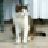
\includegraphics[height=1.5cm, align=c]{figures/carlini_wagner_orig.pdf} & 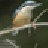
\includegraphics[height=1.5cm, align=c]{figures/carlini_wagner_adversarial.pdf} & 
\includegraphics[height=1.5cm, align=c]{figures/carlini_wagner_diff.pdf}\\
		\\
		Boundary & 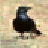
\includegraphics[height=1.5cm, align=c]{figures/boundary_orig.pdf} & 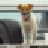
\includegraphics[height=1.5cm, align=c]{figures/boundary_adversarial.pdf} & 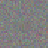
\includegraphics[height=1.5cm, align=c]{figures/boundary_diff.pdf}\\
		\\
		DeepFool & 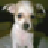
\includegraphics[height=1.5cm, align=c]{figures/deepfool_orig.pdf} & 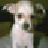
\includegraphics[height=1.5cm, align=c]{figures/deepfool_adversarial.pdf} & 
\includegraphics[height=1.5cm, align=c]{figures/deepfool_diff.pdf}\\
		\\
		Universal & 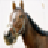
\includegraphics[height=1.5cm, align=c]{figures/universal_orig.pdf} & 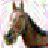
\includegraphics[height=1.5cm, align=c]{figures/universal_adversarial.pdf} & 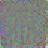
\includegraphics[height=1.5cm, align=c]{figures/universal_diff.pdf}\\
		\\
		\vspace{0.1cm}\\
	\end{tabular}
	\caption{Original images from the CIFAR10 dataset (left), adversarial images (middle) and the corresponding perturbation (right) calculated for a CapsNet.\label{tab:images}}
\end{figure}

%Universal perturbations computed for CNNs transfer very well to CapsNets. Maby CapsNet universal perturbations don't work well, because we used FGSM? Maybe the loss is to blame. Would FGSM with cross entropy loss work on the CapsNet? Or FGSM with margin loss on CNN?
%DeepFool actually seems to be a bit better for ConvNets. But the strong CW-attack fools both architecture with similarly small perturbations (Odd comparison, because CW is targeted. Maybe I should have used a untargeted CW version...)

\subsection{Visualizing Universal Perturbations}

\begin{figure}[h]
	\centering
	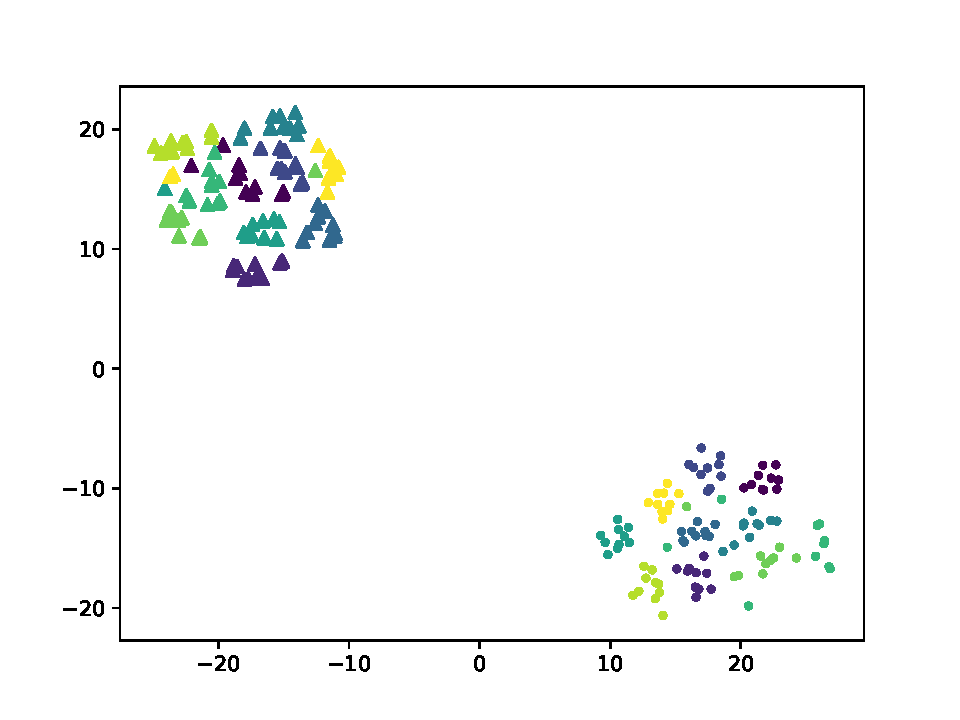
\includegraphics[height=5.5cm]{figures/tsne.pdf}
	\caption{Two dimensional embedding of the universal perturbations calculated using t-SNE \cite{tsne}. The upper right cluster represents perturbations calculated on a ConvNet, whereas the lower left cluster represents those calculated on a CapsNet. Perturbations with the same color were created using the same subset of test data.}
	\label{fig:tsne}
\end{figure}

We also visualized the universal perturbations calculated for the
CapsNet and for the ConvNet using t-SNE \cite{tsne} and we observe
that the perturbations for the CapsNet seem to be inherently different
than the perturbations for the ConvNets (see Fig.~\ref{fig:tsne}).

\section{Conclusion}
Our experiments show that CapsNets are not in general more robust to
white-box attacks. With sufficiently sophisticated attacks CapsNets
can be fooled as easily as ConvNets.  Our experiments also show that
the vulnerability of CapsNets and ConvNets is similar and it is hard
to decide which model is more prone to adversarial attacks than the
other. Moreover, we showed that adversarial examples can be transfered
between the two architectures.



% In the unusual situation where you want a paper to appear in the
% references without citing it in the main text, use \nocite
%\nocite{langley00}

\bibliography{icml}
\bibliographystyle{icml2019}



\end{document}


% This document was modified from the file originally made available by
% Pat Langley and Andrea Danyluk for ICML-2K. This version was created
% by Iain Murray in 2018, and modified by Alexandre Bouchard in
% 2019. Previous contributors include Dan Roy, Lise Getoor and Tobias
% Scheffer, which was slightly modified from the 2010 version by
% Thorsten Joachims & Johannes Fuernkranz, slightly modified from the
% 2009 version by Kiri Wagstaff and Sam Roweis's 2008 version, which is
% slightly modified from Prasad Tadepalli's 2007 version which is a
% lightly changed version of the previous year's version by Andrew
% Moore, which was in turn edited from those of Kristian Kersting and
% Codrina Lauth. Alex Smola contributed to the algorithmic style files.
